\documentclass[9pt]{article} % use larger type; default would be 10pt
\usepackage{color}
\usepackage[utf8]{inputenc} % set input encoding (not needed with XeLaTeX)
\usepackage{times}

%%% PACKAGES
\usepackage{booktabs}
\usepackage{array} 

\usepackage{amsfonts}
\usepackage{amsthm}
\usepackage{tikz}
\usepackage{amsmath}
\usepackage{float}
\usepackage{graphicx}
\usepackage{caption}
\usepackage{subcaption}
\usepackage{color}
%\usepackage{authblk}
\newtheorem{theorem}{Theorem} 
\newtheorem{lemma}{Lemma}
\newtheorem{propn}{Proposition}
\newtheorem*{thmm}{Theorem}
\newtheorem{remk}{Remark} 
\newtheorem{corol}{Corollary}
\newtheorem{definition}{Definition}



\newtheorem{thm}{Theorem}[section] 
\newtheorem{prop}[thm]{Proposition} 
\newtheorem{lem}[thm]{Lemma}
\newtheorem{cor}[thm]{Corollary} 
\newtheorem{con}[thm]{Conjecture} 

\theoremstyle{definition}
\newtheorem{defn}[thm]{Definition}
\newtheorem*{rem}{Remark}
\newtheorem*{nota}{Notation}
\newtheorem{cla}[thm]{Claim}
\newtheorem{ex}[thm]{Example}
\newtheorem{exs}[thm]{Examples}
\newtheorem*{exer}{Exercise}
\newtheorem{case}{Case}

\definecolor{sotonblue}{rgb}{0.0,0.394,0.597}
%\title{Symmetry of cerebral blood vessels: biomarker for Alzheimer's disease?}

\DeclareMathOperator{\vol}{vol}
\DeclareMathOperator{\Vol}{Vol}
\DeclareMathOperator{\Sym}{Sym}
\DeclareMathOperator{\lv}{lv}
\DeclareMathOperator{\p}{\text{Pr\"{u}fer}}
\DeclareMathOperator{\m}{m}
\DeclareMathOperator{\N}{\mathbb{N}}
\DeclareMathOperator{\Prob}{\mathbb{P}}
\DeclareMathOperator{\T}{\mathcal{T}}


\DeclareMathOperator{\F}{\mathcal{F}}
\DeclareMathOperator{\R}{\mathcal{R}}
\DeclareMathOperator{\La}{\mathcal{L}}
\DeclareMathOperator{\V}{\mathcal{V}}
\DeclareMathOperator{\Aut}{Aut}
\usepackage{amssymb}
\title{Automorphisms of Random Recursive Trees}
\author{David Matthews}
\begin{document}
\maketitle
\section{Introduction}
Graph automorphisms are essential to understanding enumerative properties of graphs.  An exact formulation of 
the number of rooted unlabelled trees is unknown \cite{harary} which emphasises the difficulty in understanding tree automorphisms.  
In addition, an intriguing 
relationship between random Fibonacci sequences and automorphism groups coming from a family of trees called random recursive 
trees \cite{macarthur2006} 
provides further motivation, if we needed any, to investigate automorphism groups of trees.  We exploit a geometric interpretation of 
a graph automorphism in which subgroups of the automorphism group are associated with certain subtrees to give bounds for the 
expected order of the automorphism group of a random recursive tree (also known as a heap-ordered tree) of order $n$. We also disprove a conjecture of MacArthur 
\cite{macarthur} which states that the automorphism group can be split in a particularly pleasing way.

In Section \ref{sec:RootedTrees} we introduce several families of increasing trees and we describe the relationship between them 
using several recursively defined functions.  In Section \ref{sec:aut} we give a geometric interpretation of the automorphism group and a 
direct product decomposition in which particular subgroups can be associated with certain subtrees. We also state MacArthur’s conjecture.  
In Section \ref{sec:func} we describe two families of recursively defined functions; inductive maps and elementary differentials and describe how these may be manipulated to calculate properties of trees such as order, path length and 
number of leaves.  In Section \ref{sec:bounds} we use inductive maps and elementary differentials to provide upper and lower bounds on the 
expected order of the order of random recursive trees.  In Section \ref{sec:disproof}  we disprove the conjecture 
of MacArthur and we make concluding remarks in Section \ref{sec:conc}.  


\section{Rooted Trees}\label{sec:RootedTrees}
 A \emph{rooted tree} is a triple $t = (r,V,E)$, such that $(V,E)$ is a finite, simple connected graph without cycles with 
 vertex set $V$ and edge set $E$ \cite{tucker}. A vertex, $r \in V$, is selected from $V$ and called the \emph{root}. By convention each edge is directed away from $r$.  We denote the
 order of a tree, $t$, by $\lvert t \rvert$ and the set of order $n$ rooted trees is denoted $\R_n$.  In addition we define 
 $R : = \bigcup R_n$.
 
 A \emph{rooted plane tree} is a quadruple $t=(r,V,E,e)$ such that $(r,V,E)$ is a rooted tree and $e$ is an embedding of $(r,V,E)$ 
 in $\mathbb{R}^2$.  The collection of order $n$ rooted plane tres is $\mathcal{F}_n$ and we define $\mathcal{F} = \cup\mathcal{F}_n$.  
 
 A \emph{labelled rooted tree} is a quadruple $t = (r,V,E,L)$ such that $(r,V,E)$ is a rooted tree and 
 \[L: V \longrightarrow S\] 
is a bijective map and $S$ is a totally ordered set (usually we set $S = \{1,2,\dots,\lvert t \rvert\}$).  We denote the set of order $n$ labelled rooted trees by $\La_n$ and we define $\La = \bigcup \La_n$.      

For any pair of vertices $u$ and $v$ of a rooted tree we write $u \leq v$ if $u$ lies on the unique shortest path from $r$ to $v$.  A 
\emph{random recursive tree} is a quadruple $t = (r,V,E,l)$ such that $t$ is a labelled rooted tree and $l$ is a labelling 
such that if $u \leq v$ then $l(u) < l(v)$. 
We denote the set of order $n$ random recursive trees by $\T_n$ and we define $\T = \bigcup \T_n$. Random recursive trees are also 
known as ``heap-ordered trees''.  

Two rooted trees $t_1$ and $t_2$ with roots $r_1$ and $r_2$ and vertex sets $V(t_1)$ and $V(t_2)$ respectively are said to be
isomorphic if there exists a bijection $f: V(t_1) \rightarrow V(t_2)$ such that 
vertices $u,v \in V(t_1)$ are adjacent if and only if $f(u),f(v) \in V(t_2)$ are adjacent and $f(r_1) = r_2$ \cite{harary}. If 
$V(t_1) = V(t_2)$ then $f$ is called a rooted tree automorphism.  The set of automorphisms of a tree, $t$, together with 
composition of maps form a group denoted $\Aut(t)$.  The order of the automorphism group is 
\[\sigma(t) := \lvert \Aut(t) \rvert,\]
notation taken from \cite{Butcher2008}. 
Consider a map $\phi: \La \rightarrow R$ that simply forgets the labels of a labelled by mapping
\[
 (r,V,E,L) \mapsto (r,V,E)
\]
The map $\phi$ is clearly surjective but not injective hence we define $\beta(t) = \lvert \phi^{-1}(t) \rvert$ to be the number of
possible isomorphism classes of labellings of a rooted tree $t \in \R$. There are $\lvert t \rvert !$ possible labellings of a tree 
$t \in \R$ hence there are  
\begin{equation}\label{eq:1}
  \beta(t) = \frac{\lvert t \rvert !}{\sigma(t)} 
\end{equation}
isomorphism classes of labellings of $t$.  

Since $\T \leq \La$ we denote by $\psi$ the restriction of $\phi$ to random recursive trees and define
\[
 \alpha(t) := \lvert \psi^{-1}(t) \rvert 
\]
The notation $\alpha(t)$ is also found in (for example) \cite{brouder,butcher1963,mazza}.  To provide a result analogous to Equation \ref{eq:1} we require several additional definitions. 

Let $t_1,t_2,\dots,t_k$ be a forest of rooted trees: the rooted tree $B^{+}(t_1,t_2,\dots,t_k)$ is built from this forest by 
introducing a new vertex, $r$ (the root of $B^{+}(t_1,t_2,\dots,t_k)$), and joining the roots of each tree $t_1,t_2,\dots,t_k$ 
to $r$ via an edge.  Since every tree $t$ ($\lvert t \rvert >1$) can be written as $B^{+}(t_1,t_2,\dots,t_k)$ we henceforth 
assume that each rooted tree $t = B^{+}(t_1,t_2,\dots,t_k)$ if $\lvert t \rvert >1$.  For convenience we will denote the rooted tree on 1 vertex 
by $\bullet$.

%%%WE can get rid of the order condition by following Connes and Kreimer and defining a rooted tree on no vertices

We have already seen one function $f: \R \rightarrow \mathbb{R}$ on rooted trees ($f(t) = \lvert t \rvert$), let us consider 
another. We define the tree factorial $t!$ recursively
\begin{align}
 \bullet! &=  1  \\
 t ! &= \lvert t \rvert \prod_{i=1}^k t_i !
\end{align}
The notation $t!$ is taken from Kreimer \cite{kreimer} because $t!$ generalises the factorial of a number.  Figure \ref{fig:1} 
provides a few examples.

\begin{figure}[H]
\centering
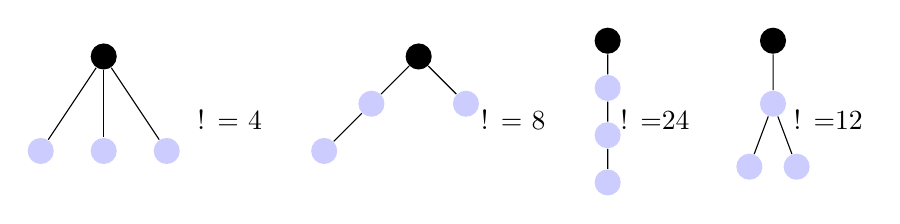
\begin{tikzpicture}
  [scale=0.8,auto=left]

  \node[style={circle,fill=black!100}] (n1) at (2,3) {};
  \node[style={circle,fill=blue!20}] (n2) at (1,1.5)  {};
  \node[style={circle,fill=blue!20}] (n3) at (2,1.5)  {};
  \node[style={circle,fill=blue!20}] (n4) at (3,1.5) {};
  \node (n5) at (4,2)  {! = 4};
  \node[style={circle,fill=black!100}] (n6) at (7,3)  {};
  \node[style={circle,fill=blue!20}] (n7) at (6.25,2.25)  {};
  \node[style={circle,fill=blue!20}] (n8) at (5.5,1.5)    {};
  \node[style={circle,fill=blue!20}] (n9) at (7.75,2.25)  {};
  \node (n10) at (8.5,2)  {! = 8};
  \node[style={circle,fill=black!100}] (n11) at (10,3.25)  {};
  \node[style={circle,fill=blue!20}] (n12) at (10,2.5)  {};
  \node[style={circle,fill=blue!20}] (n13) at (10,1.75)  {};
  \node[style={circle,fill=blue!20}] (n14) at (10,1)  {};
  \node (n15) at (10.75,2)  {! =24};
  \node[style={circle,fill=black!100}] (n16) at (12.625,3.25)  {};
  \node[style={circle,fill=blue!20}] (n17) at (12.625,2.25)  {};
  \node[style={circle,fill=blue!20}] (n18) at (12.25,1.25)  {};
  \node[style={circle,fill=blue!20}] (n19) at (13,1.25)  {};
  \node (n20) at (13.5,2)  {! =12};
  \foreach \from/\to in {n1/n2,n1/n3,n1/n4,n6/n7,n6/n9,n7/n8,n11/n12,n12/n13,n13/n14,n16/n17,n17/n18,n17/n19}
    \draw (\from) -- (\to);
\end{tikzpicture}
\caption{}\label{fig:1}
\end{figure}
Let $t = (r,V,E)$ be a rooted tree.  The \emph{induced subtree}, $t_v$, rooted at vertex $v\in V$ is the subtree of $t$ induced 
by the nodes $u$ with $v \leq u$.  

\begin{lem}\label{lem:alpha}
For a rooted tree $t$,
 \begin{equation}\label{eq:2}
\alpha(t) = \frac{\lvert t \rvert !}{t!\sigma(t)}
 \end{equation}
\end{lem}

%%%%%induced subtree

\begin{proof}
 There are $n!$ ways of labelling a tree $t \in \R_n$, however if $l$ is a random recursive labelling every induced subtree 
 $t_v$ and a totally ordered set, $S$, of labels there is precisely one possible label $s \in S$ for vertex $v$ (namely $s = \min(S)$).  
 Therefore the factor we should divide out by is precisely $t!$.  In addition, to calculate the number of isomorphism classes of 
 random recursive trees we must again divide out by $\sigma(t)$.
\end{proof}
Alternatively see \cite{Butcher2008} for a proof of Lemma \ref{lem:alpha}.
Finally, let $\chi: \F \rightarrow \R$ be the map that ``forgets'' the embedding of a rooted plane tree i.e.
\[
(r,V,E,e) \mapsto (r,V,E) 
\]
It is clear that $\chi$ 
is surjective but not injective hence we define
\[
 \gamma(t) = \lvert \chi^{-1} \rvert 
\]
the number of isomorphism classes of embeddings of a rooted tree $t$.  In order to obtain a third relation analogous to Equations 
\ref{eq:1} and \ref{eq:2} we will describe a third function $w: \R \rightarrow \mathbb{R}$ recursively:
\begin{align}
 w(\bullet) &= 1  \\ 
 w(t)  &= k!\prod_{i=1}^{k}w(t_i) 
\end{align}
  \begin{figure}[H]
\centering
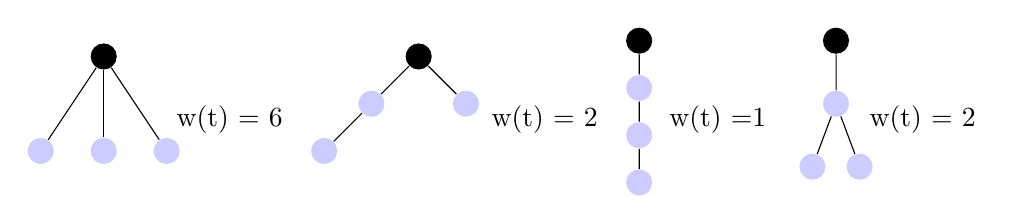
\begin{tikzpicture}
  [scale=0.8,auto=left]

  \node[style={circle,fill=black!100}] (n1) at (2,3) {};
  \node[style={circle,fill=blue!20}] (n2) at (1,1.5)  {};
  \node[style={circle,fill=blue!20}] (n3) at (2,1.5)  {};
  \node[style={circle,fill=blue!20}] (n4) at (3,1.5) {};
  \node (n5) at (4,2)  {w(t) = 6};
  \node[style={circle,fill=black!100}] (n6) at (7,3)  {};
  \node[style={circle,fill=blue!20}] (n7) at (6.25,2.25)  {};
  \node[style={circle,fill=blue!20}] (n8) at (5.5,1.5)    {};
  \node[style={circle,fill=blue!20}] (n9) at (7.75,2.25)  {};
  \node (n10) at (9,2)  {w(t) = 2};
  \node[style={circle,fill=black!100}] (n11) at (10.5,3.25)  {};
  \node[style={circle,fill=blue!20}] (n12) at (10.5,2.5)  {};
  \node[style={circle,fill=blue!20}] (n13) at (10.5,1.75)  {};
  \node[style={circle,fill=blue!20}] (n14) at (10.5,1)  {};
  \node (n15) at (11.75,2)  {w(t) =1};
  \node[style={circle,fill=black!100}] (n16) at (13.625,3.25)  {};
  \node[style={circle,fill=blue!20}] (n17) at (13.625,2.25)  {};
  \node[style={circle,fill=blue!20}] (n18) at (13.25,1.25)  {};
  \node[style={circle,fill=blue!20}] (n19) at (14,1.25)  {};
  \node (n20) at (15,2)  {w(t) = 2};
  \foreach \from/\to in {n1/n2,n1/n3,n1/n4,n6/n7,n6/n9,n7/n8,n11/n12,n12/n13,n13/n14,n16/n17,n17/n18,n17/n19}
    \draw (\from) -- (\to);
\end{tikzpicture}
\caption{}\label{fig2}
\end{figure} 
 Let $B^{+}(t_1^{n_1},t_2^{n_2},\dots,t_k^{n_k})$ denote a tree in which the root is incident to $n_1$ isomorphic copies 
 of a tree $t_1$, $n_2$ isomorphic copies of $t_2$ and so forth.  We remark that every rooted tree with at least 2 vertices can 
 be written in this way.
\begin{lem}
 \begin{equation}\label{eq:3}
  \gamma(t) = \frac{w(t)}{\sigma(t)}
 \end{equation}
\end{lem}
\begin{proof}
 %%%%%%add a diagram to this proof
 Let $B^{+}(t_1^{n_1},t_2^{n_2},\dots,t_k^{n_k})$ denote a tree in which the root is incident to $n_1$ isomorphic copies 
 of a tree $t_1$, $n_2$ isomorphic copies of $t_2$ and so forth.  We remark that every rooted tree with at least 2 vertices can 
 be written in this way.  Let $t  \in R$ and consider an induced subtree $t_v = B^{+}(t_1^{n_1},t_2^{n_2},\dots,t_k^{n_k})$. 
 Vertex $v$ contributes a factor of $\left( \sum_{i=1}^k n_i \right)! $ to $w(t)$ since it has a recursive definition.  The order of 
 automorphism group, $\sigma(t)$ can also be expressed recursively:
 \begin{align}
  \sigma(\bullet) &= 1 \\
  \sigma(t) &= n_1 ! n_2! \dots n_k ! \prod_{i=1}^k\sigma(t_i)^{n_i} 
 \end{align}
Therefore vertex $v$ contribute a factor of $\prod_{i=1}^k n_i !$ to $\sigma(t)$.  Finally consider, $\gamma(t)$, the number of isomorphism classes of embeddings of $t$.  
There are 
\[
 \frac{\left(\sum_{i=1}^k n_i \right)!}{\prod_{i=1}^k n_i!}
\]
non-isomorphic possibilities for the ordering of the children of $v$.
\end{proof}

\begin{figure}[ht]
\centering
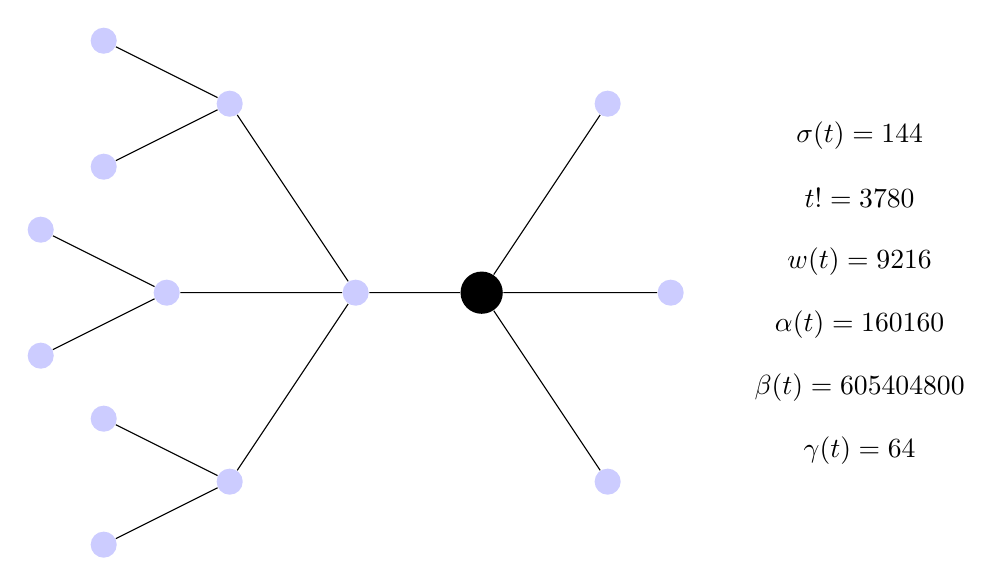
\begin{tikzpicture}
  [scale=0.8,auto=left]

  \node[style={circle,fill=black!100}](n1) at (7,5) {r};
  \node[style={circle,fill=blue!20}] (n2) at (5,5)  {};
  \node[style={circle,fill=blue!20}] (n3) at (9,8)  {};
  \node[style={circle,fill=blue!20}] (n4) at (3,2) {};
  \node[style={circle,fill=blue!20}] (n5) at (10,5)  {};
  \node[style={circle,fill=blue!20}] (n6) at (1,1)  {};
  \node[style={circle,fill=blue!20}] (n7) at (1,3)  {};
  \node[style={circle,fill=blue!20}] (n8) at (2,5)  {};
  \node[style={circle,fill=blue!20}] (n9) at (9,2)  {};
  \node[style={circle,fill=blue!20}] (n10) at (3,8)  {};
  \node[style={circle,fill=blue!20}] (n11) at (1,9)  {};
  \node[style={circle,fill=blue!20}] (n12) at (1,7)  {};
  \node[style={circle,fill=blue!20}] (n13) at (0,4)  {};
  \node[style={circle,fill=blue!20}] (n14) at (0,6)  {};
   \node (n15) at (13,7.5)  {$\sigma(t) = 144$};
   \node (n16) at (13,6.5)  {$t! = 3780$};
   \node (n17) at (13,5.5)  {$w(t) = 9216$};
   \node (n18) at (13,4.5)  {$\alpha(t) = 160160$};
   \node (n19) at (13,3.5)  {$\beta(t) = 605404800$};
   \node (n20) at (13,2.5)  {$\gamma(t) = 64$};


  \foreach \from/\to in {n1/n2,n1/n3,n1/n5,n1/n9,n2/n4,n2/n8,n2/n10,n10/n11,n10/n12,n8/n14,n8/n13,n4/n7,n4/n6}
    \draw (\from) -- (\to);
\end{tikzpicture}
\end{figure}

\section{Automorphisms of Trees}\label{sec:aut}
In this section we will describe a direct product decomposition of the automorphism group of a tree, $t$, in which factors of the direct product can be associated with particular induced subtrees of $t$.  

Recall that a (rooted) tree automorphism is a permutation of vertices that preserves adjacency and the root. In \cite{macarthur} MacArthur, 
Sanchez-Garcia and Anderson showed that an 
automorphism group, $\Aut(t)$, may be decomposed by partitioning the set of generators $S$ of $\Aut(t)$ into support-disjoint subsets 
$S = S_1 \cup S_2 \cup \dots \cup S_r$ and writing
\begin{equation}\label{eq:geometric}
 \Aut(t) = H_1 \times H_2 \times \dots \times H_r
\end{equation}
where each $H_i$ is generated by $S_i$.  This, \emph{geometric decomposition} is shown \cite{macarthur} to be unique and 
irreducible (each $H_i$ cannot be written as the direct product of support-disjoint subgroups) hence the geometric 
decomposition is well defined. We call each $H_i$ in the geometric decomposition of $\Aut(t)$ a \emph{geometric factor}. 

The reason that Equation \ref{eq:geometric} is known as a ``geometric decomposition'' is each geometric factor can be associated 
with an induced subtree.   A little more rigorously (following \cite{macarthur}), given a tree $t$ with automorphism group 
$\Aut(t)$ we define a \emph{symmetric subtree} to be the induced subtree of $t$ on the support of a geometric factor.
\begin{ex}
\begin{itemize}
 \item[(i)]  A $k$-star is an induced subtree consisting of a vertex adjacent to $k$ vertices of outdegree 0.  A $k$-star is a symmetric subtree that corresponds to a geometric factor $S_k$ (the symmetric group on $k$ objects).  
 \item[(ii)] %%%N-k stars DOOOOOOO
\end{itemize}
\begin{figure}[ht]
\centering
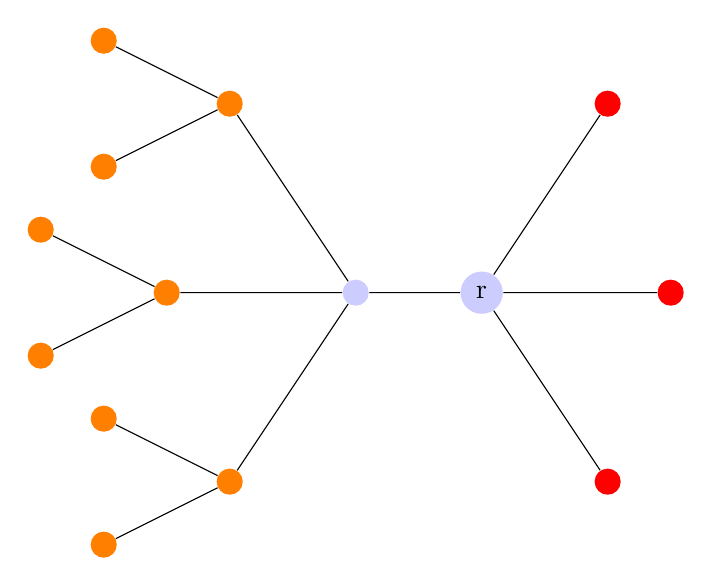
\begin{tikzpicture}
  [scale=0.8,auto=left,every node/.style={circle,fill=blue!20}]

  \node(n1) at (7,5) {r};
  \node (n2) at (5,5)  {};
  \node[style={circle,fill=red!100}] (n3) at (9,8)  {};
  \node[style={circle,fill=orange!100}] (n4) at (3,2) {};
  \node[style={circle,fill=red!100}] (n5) at (10,5)  {};
  \node[style={circle,fill=orange!100}] (n6) at (1,1)  {};
  \node[style={circle,fill=orange!100}] (n7) at (1,3)  {};
  \node[style={circle,fill=orange!100}] (n8) at (2,5)  {};
  \node[style={circle,fill=red!100}] (n9) at (9,2)  {};
  \node[style={circle,fill=orange!100}] (n10) at (3,8)  {};
  \node[style={circle,fill=orange!100}] (n11) at (1,9)  {};
  \node[style={circle,fill=orange!100}] (n12) at (1,7)  {};
  \node[style={circle,fill=orange!100}] (n13) at (0,4)  {};
  \node[style={circle,fill=orange!100}] (n14) at (0,6)  {};
  \foreach \from/\to in {n1/n2,n1/n3,n1/n5,n1/n9,n2/n4,n2/n8,n2/n10,n10/n11,n10/n12,n8/n14,n8/n13,n4/n7,n4/n6}
    \draw (\from) -- (\to);
\end{tikzpicture}
\caption{A tree, $t \in \R_n$,  rooted at $r$ such that $\Aut(t) \cong S_{3} \times S_{2}\wr S_{3}$.  
The red vertices depict a symmetric subtree (isomorphic to the leaves of a 3-star) that can be associated with the geometric factor  
of  $S_{3} \leq Aut(t)$. The orange vertices indicate a symmetric subtree that can be associated with the geometric factor $S_{2}\wr S_{3} \leq \Aut(T)$. 
In terms of Macarthur's decomposition $\mathcal{C}(t) \cong S_{2}\wr S_{3}$ and $\mathcal{E}(t) \cong{S_3}$.}
\end{figure}
\end{ex}
 It is a result of P\'{o}lya that automorphism 
groups of trees belong to the class, $\mathcal{W}$, of permutation groups which contains the symmetric groups and is closed under taking direct and wreath products.  Let $t$ 
be a rooted tree and consider the following decomposition,
\begin{equation}\label{eq:decomposition}
 \Aut(t) \cong A_1 \times A_2 \times \dots A_p \times B_1 \times B_2 \times \dots \times B_q  
\end{equation}
where each factor $A_i$ is isomorphic to a symmetric group and each $B_i$ is isomorphic to the wreath product of a group $G \in \mathcal{W}$.

By P\'{o}lya's Theorem the geometric decomposition (Equation \ref{eq:geometric}) can be written in the form,
\begin{equation}
 \Aut(t) \cong A_1 \times A_2 \times \dots A_p \times B_1 \times B_2 \times \dots \times B_q  
\end{equation}
we claim that each $A_i$ corresponds to an $(n,k)-star$ and each subgroup $B_i$ corresponds to an extended symmetric branch of 
$t$.

There is a natural way to split the geometric decomposition of $\Aut(t)$ into two subgroups. We define the direct product of symmetric groups to be the  \emph{elementary subgroup}:
\[
 \mathcal{E}(t) = A_{1} \times A_2 \times \dots\times A_p
\]
The direct product of wreath products of symmetric groups form the \emph{complex subgroup}:
\[
 \mathcal{C}(t) =  B_1 \times B_2 \times \dots \times B_q
\]
The order, $\sigma(t)$, of an automorphism group can also be split as follows:
\[
\sigma(t)  =  \lvert \mathcal{E}(t) \rvert\lvert \mathcal{C}(t)\rvert 
\]
This begs the question: does the order of either the elementary or the complex subgroup dominate the other?  

We can think of the set $\T_n$ as a probability space by choosing each tree $t \in \T_n$ equiprobably.  Given a random variable 
$X$ on the space of order $n$ random recursive trees we denote the expectation by $\mathbb{E}_{\T_n}(X)$.   

MacArthur \cite{macarthur} made the following additional conjecture:
\begin{con}\label{conj:2}
 In the limit as $n \rightarrow \infty$, 
 \[
\mathbb{E}_{\T_n}\left(  \lvert \mathcal{E}(t)\rvert^{\frac{1}{n}} \right) = C  \text{         ,         }
\mathbb{E}_{\T_n}\left(\lvert \mathcal{C}(t)\rvert^{\frac{1}{n}} \right) = 1.
\]
where $C>1$ is a constant.
\end{con}
In essense Conjecture \ref{conj:2} predicts that the subgroup of the automorphism group dominates the comples subgroup.  Geometrically, 
the contribution to $\Aut(t)$ associated with $(n,k)$-stars dominates the contribution coming from extended symmertic branches.  
   %We claim that the elementary subgroup captures the contribution that $(n,k)$-stars make to the automorphism group and the complex subgroup captures the contribution that the extended symmetric branches make to the automorphism group.  %Might Need to prove this claim%%%%%%%%%%%%%%%%%%%%
 % hence if conjecture \ref{conj:2} were true then to prove conjecture \ref{conj:1} it is enough to calculate the limiting behaviour of $(n,k)$-stars.  
%add to conclusions etc.  
\section{Functions on Trees}\label{sec:func}
In this section we will build up a tool kit of functions (called inductive maps and elementary differentials) which will be used to calculate 
 properties of rooted trees such as path length and order.  
 
\subsection{Inductive Maps}
\begin{defn}
 Let $s = \{ s_r\}_{r=0}^{\infty}$ be a sequence such that each $s_r \in \{0,1\}$.  A \emph{variety}, $\V$, of trees is a 
 collection of random recursive trees such that each vertex is permitted to have outdegree $r$ only if $s_r = 1$. 
\end{defn}
\begin{remk}
 For a more general setting see \cite{bergeron}.
\end{remk}
The \emph{degree function} associated with a sequence $s= \{ s_r\}_{r=0}^{\infty}$ is the exponential generating function (EGF) defined as follows:
\[
 \phi(w) = \sum_{r \geq 0} s_r \frac{w^r}{r!}
\]
%%%%%%%BAD Notation remove phi from earlier or here

\begin{ex}\label{ex:inductivemaps}
 The collection, $\mathcal{B}$, of increasing binary trees are the set of all random recursive trees such that each vertex has 
 outdegree either 0,1 or 2.  The degree function for increasing binary trees is
 \[
  \phi(w) = 1 + w + \frac{w^2}{2}
 \]
The degree function for random recursive trees is
\[
 \phi(w) = \exp(w).
\]
\end{ex}
Fix a variety, $\mathcal{V}$, and define $V_n$ to be the number of trees of order $n$ in $\V$.  The EGF of the variety of trees 
is 
\[
 V_{\V}(z) = \sum_{n \geq 1} V_n \frac{z^n}{n!}
\]
For example, 
\begin{align}
V_{\T}(z) &= \sum_{n\geq 1} \frac{z^n}{n} \\
&= \log\left( \frac{1}{1-z}\right)
\end{align}
since the number of random recursive trees of order $n$ is $(n-1)!$.

\begin{defn}
Let $f = \{f_n\}_{n\geq 1}$ be a sequence of real numbers.  A function $s: \R \rightarrow \mathbb{R}$ is called an 
\emph{inductive map} if it is definable by a relation,
\[
 s(t) = f_{\lvert t \rvert} + \sum_{i=1}^k s(t_i)
\]
where $t = B^{+}(t_1,t_2,\dots,t_k)$.
\end{defn}
Given an inductive map, $s$, and a variety $\mathcal{V}$ the EGF of $s$ over $\mathcal{V}$ is 
\[
 S(z) = \sum_{t \in \V} s(t) \frac{z^{\lvert t \rvert}}{\lvert t \rvert !}
\]
Let $\delta_{i,j}$ be the usual Kronecker delta. In Figure \ref{fig:3} we list possible sequences $f = \{f_n\}_{n \geq 1}$ and give the tree parameter 
 measured by the corresponding function $s$.
\begin{figure}[H]
\centering
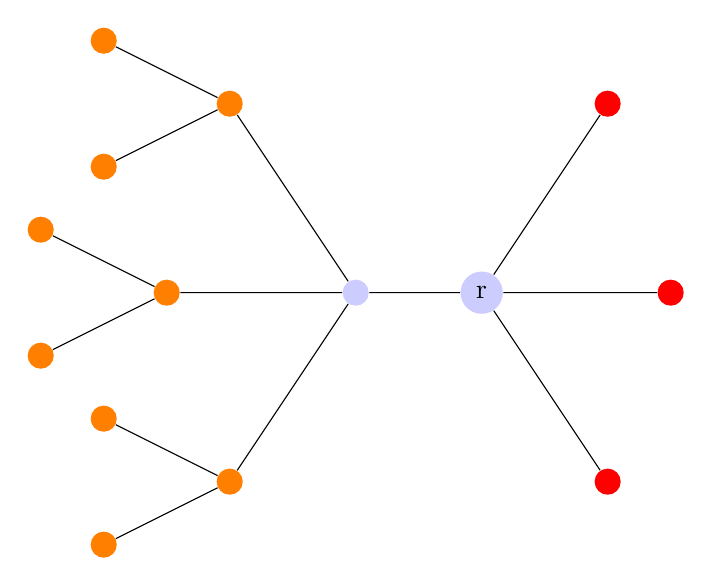
\begin{tikzpicture}
  [scale=0.8,auto=left,every node/.style={circle,fill=blue!20}]

  \node(n1) at (7,5) {r};
  \node (n2) at (5,5)  {};
  \node[style={circle,fill=red!100}] (n3) at (9,8)  {};
  \node[style={circle,fill=orange!100}] (n4) at (3,2) {};
  \node[style={circle,fill=red!100}] (n5) at (10,5)  {};
  \node[style={circle,fill=orange!100}] (n6) at (1,1)  {};
  \node[style={circle,fill=orange!100}] (n7) at (1,3)  {};
  \node[style={circle,fill=orange!100}] (n8) at (2,5)  {};
  \node[style={circle,fill=red!100}] (n9) at (9,2)  {};
  \node[style={circle,fill=orange!100}] (n10) at (3,8)  {};
  \node[style={circle,fill=orange!100}] (n11) at (1,9)  {};
  \node[style={circle,fill=orange!100}] (n12) at (1,7)  {};
  \node[style={circle,fill=orange!100}] (n13) at (0,4)  {};
  \node[style={circle,fill=orange!100}] (n14) at (0,6)  {};
  \foreach \from/\to in {n1/n2,n1/n3,n1/n5,n1/n9,n2/n4,n2/n8,n2/n10,n10/n11,n10/n12,n8/n14,n8/n13,n4/n7,n4/n6}
    \draw (\from) -- (\to);
\end{tikzpicture}
\caption{A tree, $t \in \R_n$.  Let $f = \{f_n\}$  be the sequence $f_n = 1$ for each $n \geq 1$ the corresponding inductive map, $s$, calculates the order
 of $t$ and in this case $s(t) = 14$.  Let 
$f = \{f_n\}$  be the sequence $f_n = \delta_{n,1}$ for each $n \geq 1$, the corresponding inductive map, $s$,  calculates the number of leaves of $t$ in particular 
$s(t) = 9$.}\label{fig:3}
\end{figure} 

In order to calculate $S(z)$ easily and effectively we appeal to the following Theorem of Bergeron \cite{bergeron}.
\begin{thm}\label{thm:inductivemaps}
 \[
 S(z) = Y'(z) \int_{0}^{z} \frac{F'(t)}{Y'(t)} dt
 \]
where $F(z)$ is defined from $\V$ and the sequence $f = \{f_n\}_{n \geq 1}$ as follows:
\[
 F(z) = \sum_{n \geq 0} f_n V_n \frac{z^n}{n!}
\]
\end{thm}

 \subsection{Butcher Series}
 %The reference for the beginning of this section s ``Geometric numerical integration''
 %Actually include the definition of a B-series
 Throughout this section let $f: \mathbb{R}^n \rightarrow \mathbb{R}^n$ be a suitably differentiable function and consider differential equations of the form 
 \begin{equation}\label{eq:14}
  \frac{d}{ds}{y(s)} = f(y(s))
 \end{equation}
where $y(s_0) = y_0$.  We use the notation $f'(y)$ for the derivative $\frac{d}{dy}f(y)$ and note that $f'(y)$ is a linear map (the Jacobian), the second derivative $f''(y)$ is a bilinear map and so on.   
We follow Butcher and make the following definition \cite{Butcher2008}.

\begin{defn}
Let $t = B^{+}(t_1,t_2,\dots,t_k)$ be  a rooted tree. An \emph{elementary differential} is a map  $F(t):  \mathbb{R}^n \rightarrow \mathbb{R}^n$ defined 
recursively by:
\begin{align}
 F(\bullet)(y) &= f(y) \\%%%%%This doesn't makes sense because $s$ is not a real number!!!!
 F(t)(y) &= f^{m}(y)(F(t_1)(y),\dots,F(t_k)(y))
 \end{align}
\end{defn}
\begin{ex}\label{ex:bseries}
\begin{itemize}
 \item[(i)] Suppose that $f: \mathbb{R} \rightarrow \mathbb{R}$ ($n=1$ in Equation \ref{eq:14}) is a smooth function  and that 
 $s_0 = y_0 =0$.  These kinds of expressions have been treated in great detail in \cite{butcher2008} and \cite{butcher1972}. 
 Let $f(y) = \exp(y)$ so that $f^{(m)}(y) = 1$ for $m=1,2,3,\dots$ and $F(t) = 1$ for all trees $t$. 
 \item[(ii)] Again suppose that $f: \mathbb{R} \rightarrow \mathbb{R}$ is a smooth function  and that $s_0 = y_0 = 0$.  Let 
 $f(y) = \frac{1}{1-y}$ so that $f^{(m)}(y) = m!$ for $m=1,2,3,\dots$ and $F(t) = w(t)$ for all trees $t$.
\end{itemize}   
\end{ex}

\begin{theorem}\label{Butcher}
 The solution of Equation \ref{eq:14},
 \[
  y(s) = y_0 + \int_{s_0}^{s} f(y(s')) ds'
 \]
is
\[
 y(s) = y_0 + \sum_{t \in \R} \frac{(s-s_0)^{\lvert t \rvert}}{\lvert t \rvert !}\alpha(t)F(t)(y_0)
\]
\end{theorem}
\begin{proof}
 See for example \cite{Butcher2008,brouder}
\end{proof}
\begin{ex}
 Let $f: \mathbb{R} \rightarrow \mathbb{R}$ be as in Example \ref{ex:bseries}(i).  By Theorem \ref{Butcher} the solution of 
 equation \ref{eq:14},
 \begin{equation}\label{eq:15}
  y(s) = \int_0^s \exp(y(s')) ds'
 \end{equation}
is
\begin{equation}\label{eq:16}
 y(s) = \sum_{t \in \R}\frac{s^{\lvert t \rvert}}{\lvert t \rvert !}\alpha(t)
\end{equation}
We may rewrite Equation \ref{eq:15} as the differntial equation,
\[
 y'(s) = \exp(y(s))
\]
which has solution 
\begin{equation}\label{eq:17}
 x(s) = -\log(1-s).
\end{equation}
By comparing Equation \ref{eq:16} with \ref{eq:17},
\[
 \sum_{t \in \R_n} \alpha(t) = (n-1)!
\]
which confirms the equation $\lvert \T_n \rvert = (n-1)!$.  
\end{ex}


%\subsection{Bare Green Functions} do we really need to include these????????(probably we aught to!)

\section{Bounds on the expected value of $\Aut(t)$}\label{sec:bounds}
\subsection{A lower bound}\label{sec:lower}
In this section we will calculate the expected contribution $k$-stars make to $\sigma(t)$ which is a 
lower bound for the expected value of $\Aut(t)$.  More rigorously given a  tree, $t$, any induced subtree isomorphic to a $k$-star 
can be associated with $(k-1)!$ automorphisms $\alpha \in \Aut(t)$. Let $\sigma_k(t)$ denote the total number of automorphisms 
which correspond induced subtrees isomorphic to a $k$-star in $t$ and also define
\[
  \sigma_*(t) = \sum_{k \geq 2} \sigma_{k}(t)
\]
Consider the family, $s^k$ of inductive maps over variety, $\T$, that are defined by the sequences $f^k_n = \delta_{k,n}$.  
Given a tree $t \in \T$ the inductive map $s^{k}(t)$ is the number of induced subtrees of $t$ that have order $k$ (see
Example \ref{ex:inductivemaps}). 

Following Theorem \ref{thm:inductivemaps}, to each map $s^k$ we associate the function,
\begin{align}
 F_k(z) &= \sum_{n \geq 1} f_n^k V_n \frac{z^{n}}{n!} \\
 &= \frac{z^k}{k}
\end{align}
thus $F_k'(z) = z^{k-1}$.  By Theorem \ref{thm:inductivemaps},
\begin{align}
 \sum_{t \in \T} s^k(t) \frac{z^{\lvert t \rvert}}{\lvert t \rvert !}  &= \frac{1}{1-z}\int_{0}^{z}t^{k-1}(1-t) dt \\
 &= \frac{1}{1-z}\left(\frac{z^k}{k} - \frac{z^{k+1}}{k+1} \right)  \\
 &= \frac{z^{k}}{k} + \sum_{i \geq k+1} \frac{z^i}{k(k+1)}
\end{align}
hence for $n \geq k+1$,
\[
 \sum_{t \in \T_n} s^k(t) = \frac{n!}{k(k+1)}.
\]
Let $\hat{t}_k \in \T_k$ be a random recursive tree isomorphic to a $(k-1)$-star.  Since $\hat{t}_k ! = k$ and 
$\sigma(\hat{t}_k) = (k-1)!$  Lemma \ref{lem:alpha} states that 
\[
 \alpha(\hat{t}_k) = 1
\]
hence $\hat{t}_k$ is the only (isomorphism class of) random recursive tree(s) on $k$ vertices isomorphic to a $(k-1)$-star. 
Fix $k \geq 3$ 
and suppose that $t = (r,V,E,l)$ is a random recursive tree and $t \in \T_n$ for some $n >k$.  Suppose $t$ contains an induced 
subtree, $t_v = (v,V_v,E_v,l_v)$ that has order $k$ hence $v \neq r$.  Given a set $S$ and a subset $R \leq S$ we define $\bar{R}$ 
to be the complement of $R$ in $S$.  We further define the complement of $t_v$ in $t$ to be 
\[
\bar{t_v} = (r, \bar{V_v},\bar{E_v} \backslash\{(v,f(v))\},\bar{l_v})
\]
where $f(v) \in E$ is the vertex adjacent to $v$ with a smaller label often called the father of $v$.  Notice that there exist $(k-1)!$ non isomorphic trees $t \in \T_n$ 
which consist of $\bar{t_v}$ and a random recursive tree of order $k$ joined to $\bar{t_v}$  via the edge $\{(v,f(v))\}$.

Given a tree $t \in \T$ let $n_k(t)$ be the number of induced subtrees of $t$ isomorphic to $\hat{t}_k$,
\[
 \sum_{t \in \T_n}n_k(t)  = \frac{n!}{(k+1)!}
\]
by the argument above.  Since $\sigma(\hat{t_k}) = (k-1)!$,
\begin{align}
 \mathbb{E}_{\T_n}(\log(\lvert \sigma_k \rvert^{\frac{1}{n}}) &= \frac{1}{\lvert \T_n \rvert}\sum_{t \in \T_n} \log((k-1)!^{\frac{n_k(t)}{n}}) \\
 &= \frac{1}{(n-1)!}\sum_{t \in \T_n} \log((k-1)!)\frac{n_k(t)}{n} \\
 &= \frac{\log(k-1)!}{(k+1)!}
\end{align}
By summing over all $k \geq 3$ we find that 
\[
\mathbb{E}_{\T_n}(\sigma_*(t)^{\frac{1}{n}})  = 
 \sum_{k \geq 3} \frac{\log(k-1)!}{(k+1)!}
\]
Finally, since $\exp$ is convex,  by Jensen's inequality in the limit $n \rightarrow \infty$
\[
 \exp\left(\sum_{k \geq 3}\left( \frac{\log(k-1)!}{(k+1)!} \right)\right) \leq \mathbb{E}_{\T_n}\left(\sigma(t)^{\frac{1}{n}}\right)
\]
To 5 s.f $1.0506 \leq \mathbb{E}(\sigma_*(t)^{\frac{1}{n}}$. 

\subsection{An upper bound}
In this section we will use B-series and Theorem \ref{thm:Butcher} to calculate an upper bound for the expected order 
$\mathbb{E}_{\T_n}(\sigma(t))$ of an automorphism group of a random recursive tree $t$.  

Recall from Equation \ref{eq:3} that $\gamma(t) = \frac{w(t)}{\sigma(t)}$ hence
\begin{align}
 \mathbb{E}_{\T,n}(\sigma(t))  &= \frac{1}{\lvert \T_n \rvert} \sum_{t \in R_n} \alpha(t)\sigma(t)  \\
 &< \frac{1}{\lvert \T_n \rvert} \sum_{t \in R_n} \alpha(t)w(t)
\end{align}
We define $f(s)= \frac{1}{1-s}$ as in Example \ref{ex:bseries}(ii) so that  $f^{(k)}(0) = k!$.  By Theorem \ref{Butcher} the solution to 
\begin{equation}\label{eq:5}
 y(s) = \int_0^s = \frac{1}{1-y(s')} ds'
\end{equation}
is
\begin{equation}\label{eq:7}
 y(s) = \sum_{t \in \R} \frac{s^{\lvert t \rvert}}{\lvert t \rvert !}\alpha(t)w(t)
\end{equation}
We may restate Equation \ref{eq:5} as $y'(s) = \frac{1}{1-y(s)}$ which is a first order, non-linear differential equation with 
solution
\begin{equation}\label{eq:6}
  y(s) = 1 \pm (c_1 -2s +1)^{\frac{1}{2}}
\end{equation}
where $c_1$ is a constant to be determined.  Since $x(0) = 0$ we may deduce that $c_1 = 0$.  By using the 
binomial expansion of Equation \ref{eq:6} and comparing with Equation \ref{eq:7} we find that,
\[
 \sum_{\lvert t \rvert = n}\alpha(t)w(t) = \prod_{i=1}^{n-1} (2i-1)
\]
Note that $\prod_{i=1}^{n-1} (2i-1) = (2n-3)!!$ hence using factorial identities and Stirling's approximation 
\begin{align}
 \frac{(2n-3)!!}{(n-1)!} &= \frac{(2n - 3)!}{(n-1)!^2 2^{n-1}} \\
 &~ \frac{\sqrt{\pi(n-1)}}{\pi(n-1)} \left(\frac{2(n-1)}{e} \right)^{2(n-1)} \left(\frac{e}{(n-1)} \right)^{2(n-1)} \left( \frac{1}{2} \right)^{n-1} \\
 &= \frac{\sqrt{\pi(n-1)}}{\pi(n-1)} \left( 2 \right)^{n-1}
\end{align}

Therefore,
\[
 \mathbb{E}_{\T_n}(\sigma(t)) < 2^{n-1} 
\]
By Jensen's inequality,  %%Perhaps some background on Jensen's inequality
\[
 \mathbb{E}_{\T_n}(\sigma(t)^{\frac{1}{n}}) < 2^{\frac{n-1}{n}} = \text{constant as required}
\]
%It is interesting to compare the expected value of $\sigma(t)^{\frac{1}{n}}$ with the typical value of $\sigma(t)^{\frac{1}{n}}$ 
%for random recursive trees since this will illuminate the nature of the distribution of automorphism group orders.  
 
%Consider the following alternative decription of random recursive trees as a growing tree process:  A \emph{random recursive 
%tree}, $ t \in \T_n$ can be written as a nested sequence of random recursive trees:
%\[t = t^1 \subset t^2 \subset \dots \subset t^n.\]
%such that at initial time $s=1$ the tree $t^1$ is the random recursive tree with 1 vertex and no edges and subsequently at times 
%$s = 2,3,\dots,n$ a vertex, $v$, is chosen from the set vertices, $V^{(s-1)}$, of tree $t^{(s-1)}$ uniformly at random and a 
%new vertex labelled $t$ is attached to $v$ via an edge.  
%\begin{remk}
% The interpretation, above, makes it clear why we name this family; \emph{random} recursive trees.  It also makes obvious the 
% observation that $\lvert \T_n \rvert  = (n-1)!$ since at time $s$ there are $s-1$ possible vertices for $v$ to be attached.  
%\end{remk}
%Let $t = \{t^s\}_{s\geq 1}$ be a random recursive tree and $X_{s,i}$ be the number of vertices of outdegree $i-1$ in $t^s$.
 
%\begin{thm}
% In the limit as $s \rightarrow \infty$, almost surely $\frac{X_{s,i}}{s} \rightarrow 2^{-(i+1)}$. 
%\end{thm}
%\begin{proof}
% See Janson \ref{}
%\end{proof}
%As a corollary to this, in the limit as $s \rightarrow \infty$, almost surely $\frac{X_{s,i}}{s} \rightarrow 2^{-(i+1)}$. 
%%Be careful....might have already done the hard work....
\section{A disproof of Conjecture \ref{conj:2}}\label{sec:disproof}
In this section we will disprove Conjecture \ref{conj:2} by demonstrating that there exists a subset, $S\subset\mathcal{C}(t)$, such 
that the expected order of $S$ in $\T_n$ grows exponentially with $n$.  In particular, let 
$\tilde{t}$ be the tree on 7 vertices shown in Figure \ref{fig:7} and notice that every induced subtree of tree $t$ isomorphic to 
$\tilde{t}$ is contained in the support of a geometric factor $H_i \leq \mathcal{C}(t)$. %%Add figure 
Let $\sigma_{\tilde{t}}(t)$  be the number of automorphisms $\alpha \in \Aut(t)$ that correpond to $\tilde{t}$.  
\begin{figure}[H]
\centering
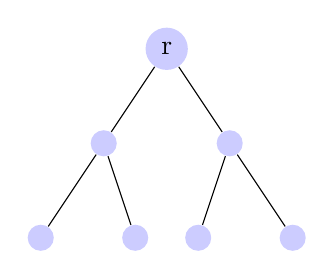
\begin{tikzpicture}
  [scale=0.8,auto=left,every node/.style={circle,fill=blue!20}]
  \node(n1) at (3,4) {r};
  \node (n2) at (2,2.5)  {};
  \node(n3) at (1,1)  {};
  \node (n4) at (2.5,1) {};
  \node (n5) at (4,2.5)  {};
  \node (n6) at (3.5,1)  {};
  \node (n7) at (5,1)  {};
 \foreach \from/\to in {n1/n2,n1/n5,n2/n3,n2/n4,n5/n6,n5/n7}
    \draw (\from) -- (\to);
\end{tikzpicture}
\caption{Tree $\tilde{t}$}\label{fig:7}
\end{figure} 

Consider the inductive map, $s$  (over the variety $\T$) defined by a sequence $f_n = \log(8)\delta_{n,7}$ and assume that $s$ has EGF
\begin{equation}\label{eq:9}
  S(z) = \sum_{t \in \T} s(t)\frac{z^{\lvert t \rvert}}{\lvert t \rvert !}
\end{equation}
Since $s$ is just the $s^k$ defined in Section \ref{sec:lower} for $n \geq 8$,
\begin{equation}\label{eq:10}
 S(z) = \sum_{n \geq 8} \frac{z^n}{56}
\end{equation}
\[
 \sum_{t \in \T_n}s^k(t) = \frac{n!}{56}
\]
Given a random recursive tree $t$ let $\epsilon(t)$ denote the number of induced subtrees of $t$ that are isomorphic to 
$\tilde{t}$. Since $\alpha(\tilde{t}) = 10$ and $\lvert \T_7 \rvert = 6!$ and $\sigma(\hat{t}) = 8$ 
following a similar argument to Section \ref{sec:lower} 
we may write,
\[
 \sum_{t \in \T_n}\log(8)\epsilon(t) = \frac{10\log(8)n!}{8!}
\]
Therefore the expected value, 
\begin{align}
 \mathbb{E}_{\T_n}\left(\log\left(\sigma_{\tilde{t}}(t)^{\frac{1}{n}}\right)\right) &= \frac{1}{\lvert \T_n \rvert}\sum_{t \in \T_n} \log\left(8^{\frac{\epsilon(t)}{n}}\right) \\
 &= \frac{1}{(n-1)!}\sum_{t \in \T_n} \frac{\log(8)\epsilon(t)}{n} \\
 &= \frac{10\log(8)}{8!}
\end{align}

Since exponential is a convex function,
\[
 1 < \exp\left( \frac{10\log(8)}{8!}\right) \leq \mathbb{E}_{\T_n}\left(\sigma_{\tilde{t}}(t)^{\frac{1}{n}}\right) \leq \mathbb{E}_{\T_n} \left( \lvert \mathcal{C}(t) \rvert^{\frac{1}{n}}   \right)
\]
by Jensen's inequality; thus disproving Conjecture \ref{conj:2}.  
\section{Conclusions}\label{sec:conc}

\bibliographystyle{amsalpha}
\bibliography{Bounds.bib}

\end{document}
